
\documentclass[xcolor={dvipsnames}]{beamer}
\usepackage{amsmath,amsfonts,amssymb,pxfonts,eulervm,xspace}
\usepackage{graphicx}
 \usepackage{multimedia}
\usepackage{media9}
\usepackage{minted}

\usepackage{animate}

\graphicspath{{./figures/}}
\usetheme{ccnycrest}


\newenvironment{changemargin}[2]{%
\begin{list}{}{%
\setlength{\topsep}{0pt}%
\setlength{\leftmargin}{#1}%
\setlength{\rightmargin}{#2}%
\setlength{\listparindent}{\parindent}%
\setlength{\itemindent}{\parindent}%
\setlength{\parsep}{\parskip}%
}%
\item[]}{\end{list}}

\begin{document}

\title{ CS102: While and Do While Loops }
\author{Hannah Aizenman}
\date


\begin{frame}
	\titlepage
\end{frame}

\begin{frame}{Print one line?} 
	\begin{figure}
		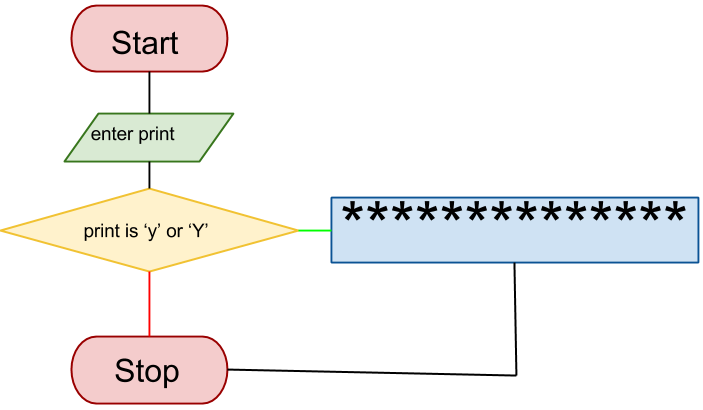
\includegraphics[width=1\textwidth]{if_line}
	\end{figure}
\end{frame}

\begin{frame}[fragile]{Print one line?}
\large
\begin{minted}{c++}
#include <iostream>

int main(){
    char print;
    cout<<"Print line?"<<endl;
    cin>>print;
    if(print== 'y' || print =='Y'){
       std::cout<<"**************"<<std::endl;
    }
    return 0;
}
\end{minted}
\end{frame}


\begin{frame}{Print one line? More?}
	\begin{figure}
		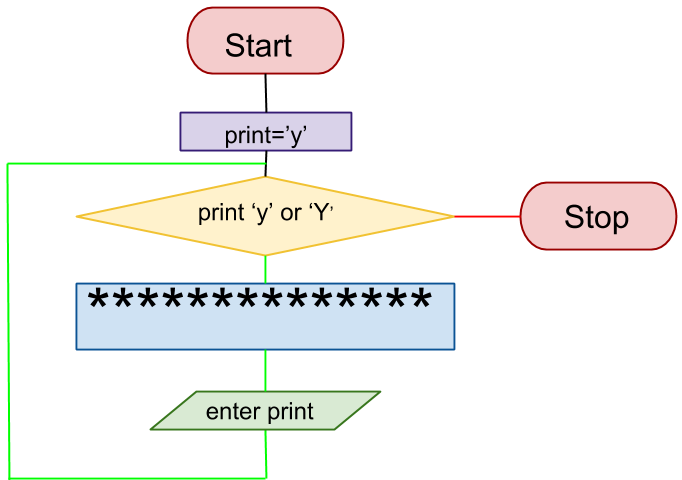
\includegraphics[width=1\textwidth]{while_line}
	\end{figure}
\end{frame}

%
\begin{frame}[fragile]{Print one line? More?}
\large
\begin{minted}{c++}
int main(){
    char print;

    std::cout<<"Print line? "<<std::endl;
    std::cin>>print;

    while(print == 'y' || print =='Y'){
        std::cout<<"**************"<<std::endl;
        std::cout<<"Print line? "<<std::endl;
        std::cin>>print;
    }
return 0;
}
\end{minted}
\end{frame}

\begin{frame}{Practice While Loops}
\begin{enumerate}
	\item Write a program that reads numbers until number is less than or equal to 100.
	\item Find the minimum of the numbers being read in. 
	\item Find the maxmium.
	\item Find the average.
\end{enumerate}
\end{frame}

\begin{frame}{Print another line?}
	\begin{figure}
		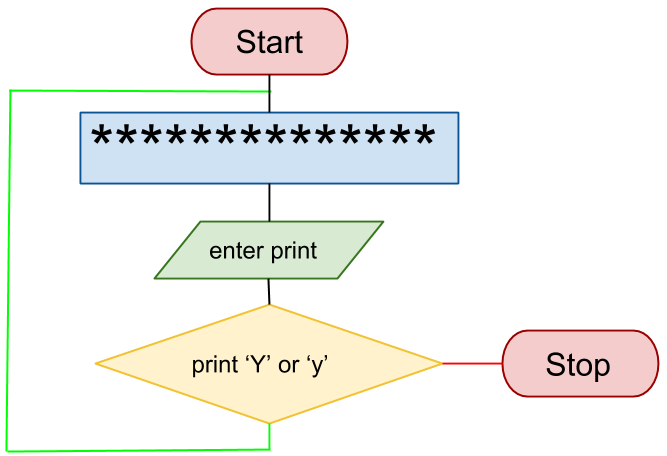
\includegraphics[width=1\textwidth]{do_while_line}
	\end{figure}
\end{frame}

\begin{frame}[fragile]{Print another line?}
\large
\begin{minted}{c++}
int main(){
    char print;

    do{     
        std::cout<<"**************"<<std::endl;
        std::cout<<"Print line? "<<std::endl;
        std::cin>>print;
    }while(print == 'y' || print =='Y');

 return 0;
}
\end{minted}
\end{frame}

\begin{frame}{Practice Do While Loops}
\begin{itemize}
	\item Machine epsilon is the smallest positive floating point number such that 1.0 + machine epsilon is not equal to 1.0. Epsilon can be approximated by repeatedly dividing a number by 2. Write a program to calculate epsilon. 
	\item
\end{itemize}
\end{frame}

\begin{frame}{Break out of Loop}
	\begin{figure}
		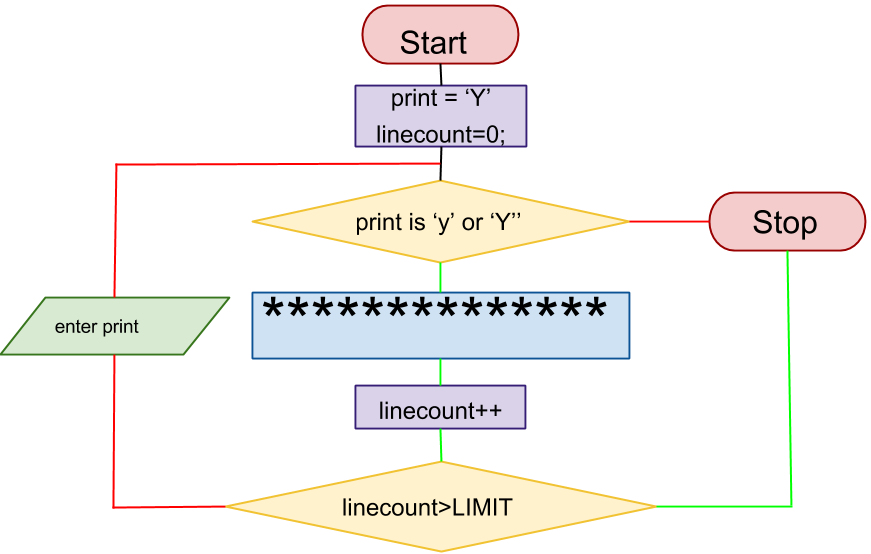
\includegraphics[width=1\textwidth]{break_line}
	\end{figure}
\end{frame}

\begin{frame}[fragile]{Break Statement}
\begin{minted}{c++}
const int LIMIT = 100;
char print= 'y';
int linecount = 0;

std::cout<<"Print a line?"<<std::endl;
std::cin>>pretzel;

while(print == 'y' || print =='Y'){
    std::cout<<"**************"<<std::endl;
    linecount++;
    if(linecount>LIMIT){
        break;     
    }
    std::cout<<"Print line? "<<std::endl;
    std::cin>>print;
}
\end{minted}
\end{frame}

\begin{frame}{Print 100, then ask}
	\begin{figure}
		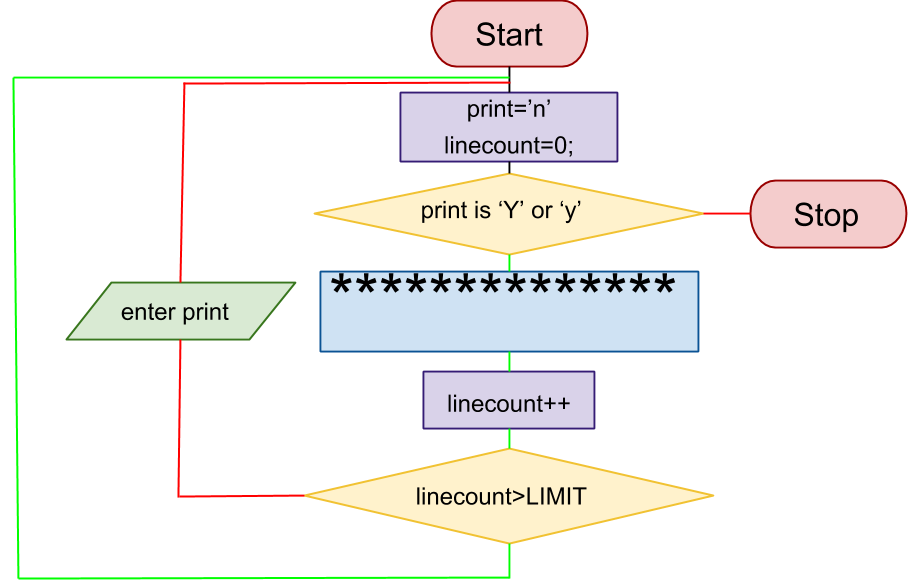
\includegraphics[width=1\textwidth]{continue_line}
	\end{figure}
\end{frame}


\begin{frame}[fragile]{Continue Statement}
\begin{minted}{c++}
const int LIMIT = 100;
char print= 'y';
int linecount = 0;

std::cout<<"Print a line?"<<std::endl;
std::cin>>pretzel;

while(print == 'y' || print =='Y'){
    std::cout<<"**************"<<std::endl;
    linecount++;
    if(linecount<LIMIT){
        continue;
    }
    std::cout<<"Print line? "<<std::endl;
    std::cin>>print;
}
\end{minted}
\end{frame}

\begin{frame}[fragile]{Infinite Loops}
	\begin{description}
	\item[no range]
	\begin{minted}{c++}
		for(;;){std::cout<<"hello";}
	\end{minted}

	\item[always true]
	\begin{minted}{c++}
		while(true){std::cout<<"world";};
	\end{minted}
	\item[always true]
	\begin{minted}{c++}
		do{std::cout<<"!"<<std::endl;}while(1);
	\end{minted}

	\item[k \& i increase]
	\begin{minted}{c++}
	     k=10;
	     for(int i=0; i<k; i++){k+=i};
	\end{minted}

	\item[always i \textgreater 0]
	\begin{minted}{c++}
	     int =10;
	     while(i>=0){i/=2};
	\end{minted}
	
	\item[no change]
	\begin{minted}{c++}
	     stop = 'N'
	     do{std::cout<<"quit";}{while{stop!='Y'};
	\end{minted}

	\end{description}
	
\end{frame}

\end{document}

